\documentclass[MiniProjectMain]{subfiles}
\begin{document}

\chapter{Implementation}
\section{Encoder}
lorem ipsum
\begin{lstlisting}[caption=Cyclic encoding]
function [ codeVector ] = cyclicEncode( genPol, messageVector )
% Returns a code vector, given a meassage vector and a cyclic 
% generator polynomial.
% genPol is a generator polynomial in polynomial form.
% messageVector a is in binary form.
% codeVector is the encoded vector in binary for

r = degree(genPol);
k = numel(messageVector);
n = k + r;
% Convert the generator polynomial to vector form.
genVec = pol2polvec(genPol);
% Calculate the generator matrix in systematic form.
[H,G] = cyclgen(n, genVec,'system');
% Encode the meassage vector.
codeVector = rem(messageVector * G,2);
end
\end{lstlisting}


\section{Meggit decoder}

\begin{lstlisting}[caption=Cyclic Meggit decoding]
function [ codeVector, errorVector, tag, bufferReg, syndromeReg ] 
= cyclicDecode( receiveVector, genPol, n, k)
% Meggit Decoder

r = degree(genPol);
n1 = numel(receiveVector);
k1 = n1-r;
if(n1 ~= n || k1 ~= k)
   error('The received vector and the generator polynomial does 
   not correspond to the values of n and k'); 
end

% Generator polynomial in vector form:
genVec = pol2polvec(genPol);

% 'Registers' initialization:
bufferReg = zeros(1,n); % Buffer register
codeVector = zeros(1,n); % Corrected output
errorVector = zeros(1,n); % Calculated errors
syndromeReg = zeros(1,r); % Syndrome register
errorDetected = 0; % Error detection 'gate'
tag = 'Not set'; % Correctable/Uncorrectable tag.
% Syndrome vector table used for comparison with the syndromeReg
errSyndTable = generateErrExpr(n, genPol);

for i = 1:n*2
    % Output codeVector shifting
    codeVector = circshift(codeVector,[1 1]);
    % Only output result after the received vector is shifted 
   	% into the buffer.
    if(i > n)
        codeVector(1) = mod(bufferReg(end) + errorDetected,2);
    end

    %Update syndrome register:
    syndromeGate = syndromeReg(end);

    % SyndromeGate feedback and shifting:
    for j = 1:r-1
        syndromeReg(r+1-j) = mod(syndromeReg(r-j) 
        					+ syndromeGate*genVec(r+1-j),2);
    end
    
    % The errorDetected feedback is only used after the buffer 
    % have been filled:
    if(i > n)
        syndromeReg(1) = mod(receiveVector(n) + errorDetected 
        				+ syndromeGate*genVec(1),2);
    else
        syndromeReg(1) = mod(receiveVector(n) 
        				+ syndromeGate*genVec(1),2);
    end
    
    % Compare syndrome register with syndrome vector table:
    for j = 1:n
        if(isequal(errSyndTable(j,:),syndromeReg))
            errorDetected = 1;
            if(i >= n)
                errorVector(2*n-i) = 1;
            end
            break;
        end
        errorDetected = 0;
    end

    % Buffer register shifting and feedback:
    bufferReg = circshift(bufferReg,[1 1]);
    bufferReg(1) = mod(receiveVector(n) + codeVector(1),2);
    
    % Receive vector shifting:
    receiveVector = circshift(receiveVector,[1 1]);
    receiveVector(1) = 0;
end
% Update tag:
if(isequal(syndromeReg,zeros(1,r)))
    tag = 'Correctable';
else
    tag = 'Uncorrectable error';
end
end
\end{lstlisting}

\begin{lstlisting}[caption= Generation of error syndrome vectors.]
function [ errSynd ] = generateErrExpr( n, genPol )
% Returns the syndrome vectors, used in a Meggigt decoder for a 
% double-error correcting generator polynomial.
% errSynd = generateErrExpr( n, genPol )

% The degree of the generator polynomial is equal to the length 
% of the syndrome vectors.
r = degree(genPol);
% Convert the generator polynomial to vector representation.
genVec = pol2polvec(genPol); 
% Calculate the parity check matrix in systematic form.
H = cyclgen(n, genVec,'system');
% Possible error vectors used in the Meggit decoder
e = eye(n);
e(:,n) = 1;
%Syndrome vector matrix
errSynd = zeros(n,r);
for i = 1:n
    % syndrome = e*H';
    errSynd(i,:) = mod(e(i,:)*H',2);
end
end
\end{lstlisting}

\section{Helper functions}
\begin{lstlisting}[caption=Maximum degree of polynomial]
function d = degree(eq)
% Returns the maximum degree of the input equation.
% d = degree(eq)
% Note: Only accepts an equation with elements with only one '^'.
a = strtrim(strsplit(char(eq),'+'));
d = 0;
for i=1:length(a)
    f = strsplit(char(a(i)),'^');
    if length(f) == 2
        if d < double(sym(f(2)))
            d = double(sym(f(2)));
        end
    end
end
end
\end{lstlisting}


\begin{lstlisting}[caption=Convert polynomial to vector form.]
function polvec = pol2polvec(Pol,n)
% Returns the polynomial representation of a symbolic polynomial as a vector.
% The polynomial vector is ascending(left to rigth).
% polvec = pol2polvec(Pol) returns a polynomial vector.
% polvec = pol2polvec(Pol,n) returns a vector of length n, if
% n > length(pol2polvec(Pol))

switch(nargin)
    case 2
        polvec = rot90(sym2poly(Pol),2);
        polvec = [polvec zeros(1,n-length(polvec))];
    case 1
        polvec = rot90(sym2poly(Pol),2);
end
\end{lstlisting}

\section{Graphical User Interface}

\begin{figure}[H]
\begin{center}
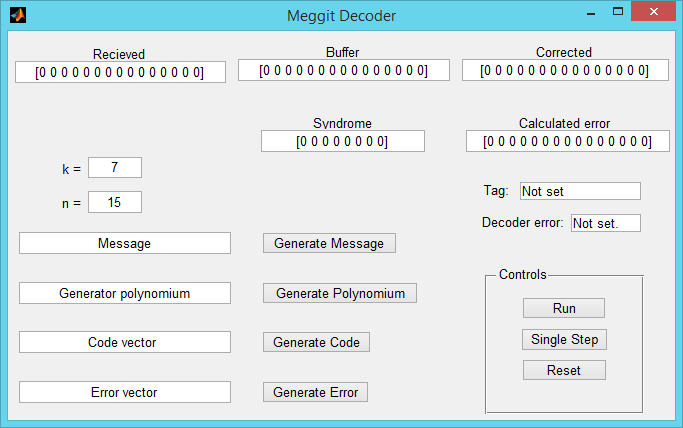
\includegraphics[width=\textwidth]{GUI}
\end{center}
\end{figure}

\end{document}
